\chapter{Einführung in die Programmierung eines EEXCESS--Clients}
\section{Grundlegendes}
Die Kommunikation eines Clients mit dem EEXCESS--Server basiert auf
dem Austausch von JSON--Objekten. Im Rahmen des
\SECH--Browser--Projektes werden nur die Dienste des
Privacy--Proxy--Service\footnote{Im Folgenden mit PP--Service
  abgekürzt.}  in Anspruch genommen. Die dafür benötigten
JSON--Objekte sind in der Online--Dokumentation des EEXCESS--Projektes
auf GitHub beschrieben.

\section{Informationsanfrage}
Informationsanfragen an den PP--Server geschehen in der Regel in zwei
Schritten.

\begin{figure}[ht]
    \centering
    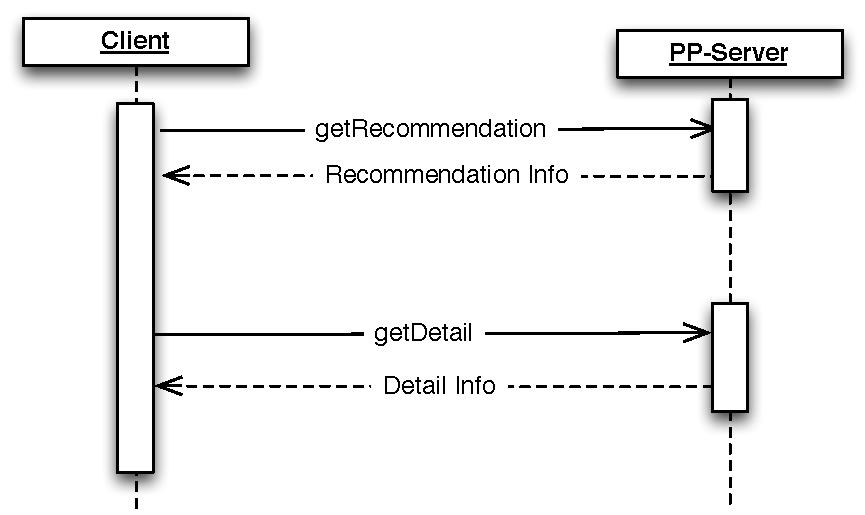
\includegraphics[width=0.75\textwidth]{clientServerComm}
    \caption{Beispiel für Informationsanfrage an den EEXCESS PP--Service}
    \label{fig:clientServerEEXCESS}
\end{figure}

Im ersten Schritt wird eine durch Suchparameter beschriebene
\Verb|/recommend|--Anfrage an der Server gestellt. Die Antwort darauf
besteht aus einem JSON--Objekt. Es enthält, neben den eigentlichen
Ergebnissen der Suchanfrage, auch eine eineindeutige ID zur späteren
Referenzierung der Anfrage. Die zurückgelieferten Ergebnisse bestehen
ihrerseits wieder aus verschiedenen Elementen, unter anderem einem
Titel der das Element näher beschreibt, einer URI die angibt wo das
Objekt gespeichert ist und einer eineindeutigen ID zur Referenzierung
des Objekts. Diese Informationen würden bereits ausreichen, um die einzelnen
Ergebnisse der Suchanfrage aus dem Netz zu laden. Da der Benutzer aber
selber entscheiden soll, ob die angezeigten Zusatzinformationen für
ihn interessant sein könnten, muss er vor der Darstellung eine Auswahl
treffen können. Dies ist anhand des Titels in der Regel nur schwer
möglich!

In einem zweiten, optionalen Schritt kann daher für jedes Ergebnis
einer \Verb|/recommend|--Anfrage eine detaillierte Kurzbeschreibung
vom PP--Server abgerufen werden. Der dafür vorgesehene
\Verb|/getDetails|--Befehl übergibt die ID der Suchanfrage und die
\Verb|documentBadge|--Informationen des ursprünglichen Ergebnisses an
den PP--Server und bekommt, falls bei der Datenquelle hinterlegt, eine
Kurzbeschreibung des Ergebnisses. An Hand dieser Kurzbeschreibung kann
der Anwender dann entscheiden, ob das eigentliche Informations--Objekt
über die zugeordnete URI geladen werden soll oder nicht.

\subsection{\texttt{/recommend}--Anfrage im \SECH--Browser Projekt}
Ein minimales JSON--Objekt für eine \Verb|/recommend|
Anfrage an den PP--Server besteht aus 3~Teilen:
\begin{enumerate}
     \item Den \Verb|origin| Informationen, die den Client näher beschreiben.
     \item Dem \Verb|loggingLevel|, der angibt ob der PP--Server die
    Anfragen aufzeichnen darf oder nicht.
    \item Den \Verb|contextKeywords|, die die eigentlichen
   Suchbegriffe beinhalten.
\end{enumerate}

Über weitere Parameter können die \Verb|/recommend|--Anfrage noch
genauer definiert werden. Im \SECH--Browser werden folgende
Parameter verwendet:
\begin{enumerate}
     \item \Verb|numResults|, um die Anzahl der vom PP-Server
    zurückgegebenen Resultate begrenzen zu können.
     \item Das \Verb|isMainTopic| Attribut der \Verb|contextKeywords|
    Einträge, um bei mehreren Suchparametern eine Priorisierung
    durchführen zu können.
     \item \Verb|interests|, um die Anfragen genauer an die Vorlieben
    des Benutzers anpassen zu können.
     \item \Verb|languages|, um bevorzugt \SECH--Annotations in der
    Muttersprache des Benutzers zu verwenden.
     \item \Verb|timeRange|, um die \SECH--Annotations zeitlich
    eingrenzen zu können.
\end{enumerate}

%Falls vom PP--Server unterstützt, sollen auch folgende Parameter zur
%näheren Beschreibung der Suchanfrage verwendet werden:
%\begin{itemize}
%     \item \Verb|ageRange|
%     \item \Verb|gender|
%     \item \Verb|address|
%\end{itemize}